\section{Effect of an azimuthal field}\label{result3}
In this section we add an azimuthal field so that $B_y\neq 0$,  
parameterized by $\epsilon \equiv B_y/B_z$. However, we continute to
use $B_z$ for normalizations and $\beta$ is associated with the
vertical Alfven speed. We also extend the previous calculations to the
full disk $z\in[-Z_s,Z_s]$, which allows us to compare the effect of
self-gravity on MRI modes with different symmetries across the
midplane. 

\subsection{Ideal disks without GI} 
Here we consider an isothermal disk with $Q=0.2$
($Q_\mathrm{2D}=0.72$) and $\beta=10$ in the limit of ideal MHD
($\Lambda_0=100$). Gravitational instability is not expected because 
Fig. \ref{compare_growth3} shows that even for $Q=0.18$, GI is 
surpressed for $\beta \lesssim 15$. We consider azimuthal field
strengths with $\epsilon=[0,3]$. 

Fig. shows the MRI growth rates for the above system as a function of
$k_x$. The top panel are modes with even midplane symmetry: 
$W^\prime(0)\sim 0$ for $k_x\to0$, and the bottom panel are modes with odd midplane 
symmetry: $W(0)\sim 0$ for $k_x\to0$. The latter set of modes were 
excluded in the previous sections by midplane boundary 
conditions. The plot also include growth rates computed in the Cowling
approximation. As expected, none of the modes are energetically
dominated by self-gravity, $\avg{E_g}<\avg{E_m}$. 

%general stabilization of MRI

\begin{figure}
  \includegraphics[width=\linewidth,clip=true,trim=0cm 2cm 0cm 0cm]{figures/compare_growth3_tilted_even.ps} 
  \includegraphics[width=\linewidth,clip=true,trim=0cm 0cm 0cm 0.52cm]{figures/compare_growth3_tilted_odd.ps}
  \caption{Growth rates in massive isothermal disks with $Q=~0.2$ and
    $\beta=10$ for a range of azimuthal field strengths $B_y/B_z$. The
    dots are solutions computed from the full problem, with the
    colorbar measuring the gravitational potential perturbation, while
    the solid curves are computed from the Cowling approximation. The
    top panel correspond to even modes and the
    bottom panel correspond to odd modes, which have
    $W^\prime(0)\sim0$ and $W(0)\sim0$, respectively, for $k_x\to0$.
    \label{compare_growth3_tilted}}
\end{figure}

%We consider $\epsilon\equiv B_y/B_z \in[0,3]$. The 

Consider first the even modes in the top panel of
Fig. \ref{compare_growth3_tilted}. Self-gravity slightly stabilizes
modes with small $k_x$ as $B_y$ is increased. SG destabilizes modes
with  $k_xH\gtrsim O(1)$, and is most effective for purely
vertical fields: for $\epsilon=0,\, k_xH\simeq 1.4$, SG increases the
growth rate by $\sim 30\%$. Consequently the cut-off wavenumber is
larger when SG is included. This destabilization effect weakens with
$B_y$ because the total magnetic pressure increases, which generally
opposes GI, although the modes are fundamentally associated with MRI.  


The odd modes in the bottom panel of Fig. \ref{compare_growth3_tilted} 
display opposite behavior. Self-gravity has negligible effect when 
the field is purely vertical ($B_y=0$). SG stabilizes all wavelengths,
and is most effective with increasing $B_y$ and $k_xH =  O(1)$. 


%With $B_y\neq 0$, the MRI is compressible even in the Cowling
%approximation \citep{pessah05}.   

\begin{figure}
  \includegraphics[width=\linewidth,clip=true,trim=0cm 1.5cm 0cm
    0cm]{figures/result_tilted_cowling.ps}  
  \includegraphics[width=\linewidth,clip=true,trim=0cm 0cm 0cm
    0.cm]{figures/result_tilted_fullsg.ps} 
  \caption{caption
    \label{result_tilted}}
\end{figure}


\subsection{Resistive disks with GI}


%\subsection{GI}

